\documentclass[pageno]{jpaper}

\newcommand{\IWreport}{Spring 2019}
\newcommand{\quotes}[1]{``#1''}


\widowpenalty=9999

\usepackage{graphicx}
\usepackage[normalem]{ulem}
\useunder{\uline}{\ul}{}
\graphicspath{ {./../Analysis/} }
\begin{document}

\title{Measuring Musical Sampling Impact Through Network Analysis}

\author{Justin Tran\\Adviser: Andrea LaPaugh}

\date{}
\maketitle

\thispagestyle{empty}
\doublespacing
\begin{abstract}
Musical sampling influence has only recently been studied through network structures through the basic analysis of artist-artist sampling relationships. In this paper, I integrate the use of additional properties of music sampling (such as genre, time period, and audio element sampled) to investigate patterns of influence in the musical community at large. Using the WhoSampled dataset, I investigate statistical metrics such as the most-sampled artists songs as well as the trend for musical sampling over time. I also take a more nuanced look at "influence" by providing a variety of graph centrality measurements for determining the influence of a node (representing an artist) on other nodes. This analysis resulted in a greater understanding of musical influence certain artists and genres had over other heavily-sampling artists and genres over time. The most influential genre was found to be Funk/Soul/Disco while the most influential artist of all time was James Brown. More specific influencers from different time periods were also found. We conclude with possible future research that can be applied to this network analysis of musical sampling.
\end{abstract}

\section{Introduction}
Music sampling is the act of taking a portion of another musical piece and reusing it as an element in a new recording. Musical sampling dates as far back as the 1890’s which suggest that sampling may be a product of stylistic practices rather than being a modern trend. While certain genres of music are notable for utilizing sampling heavily during certain eras such as early 90’s hip-hop, the use of sampling has spread far beyond hip-hop and is being employed by a variety of music producers across a variety of genres.

Sampling will be the measure of musical influence in this paper. Specifically, influence will be partially defined by the number of times a piece is sampled by other pieces. Sampling informs listeners of the artist’s level of influence on other musicians within their expected sphere of influence within a genre or outside of it. With this in mind, we can ask, "Are there certain musicians or genres that exhibit a strong influence on others in the music community?" 

The primary goal of this paper is to explore relationships between artists and genres and determine which utilize sampling the most in comparison to others. In addition, we can observe intra-genre and inter-genre sampling (having a sample be used by an artist from the same genre versus another genre, respectively). By noting the intra-genre relationships, we can identify whether artists tend to sample more from other artists within their genre or if they tend to extend their musical reach to unrelated genres instead. 
The secondary goal is to apply our network analysis on the sampling patterns of audio element (sample vocals, bass lines, drum beats, etc.) sampling across genres to different time periods. This time-based model of analyzing sampling can uncover specific sampling practices that arose during certain eras or possibly failed to exist after a certain period, an aspect of musical sampling that is often unconsidered in past related works.
\subsection{Sampling Influence and Copyright Law}
The importance of musical sampling influence takes on a controversial role in modern music due to the variety of lawsuits arising from unrestricted use of samples. Somoano notes that  parties filing lawsuits for uncondoned sampling usage often cite the fact that their music has grealy influenced the music community to bolster the argument behind the importance of the possession of their song as billable property. \cite{Somoano} We can interpret these statements as saying that their sampling influence in the music community is both culturally noticeable and quantitatively measurable. By charting musical influence patterns with sampling based on a variety of factors such as time period, genre, and audio element sampled, one can better understand the artists and record companies filing lawsuits for uncondoned uses of a sample and observe whether their record does have a large influence on specific musical communities. 
\section{Related Work}
\subsection{Musical Sampling Influence Networks using WhoSampled}
In past works, research has been performed on basic network analysis of sampled music that is grouped into genres at the very least. This is seen in
a paper by Bryan and Wang from Stanford University’s Department of Music. \cite{Bryan} The paper utilized the WhoSampled.com dataset to analyze musical influence and rank artists, songs, and genres based on their level of “sampling influence” throughout history then proceeded to rank the categories based on their amount of sampling analyzed via clustering and node degree. Overall, network analysis was used to indicate the relative flow of samples between genres. However, no intra-genre analysis was included which limited the potential findings that this dataset gives access to. The paper noted the complex nature of using network analysis to define "influence" in music but settled on using degree centrality as a sole measure of influence. They came to the conclusion that a unique power-law degree distribution is followed in the musical sampling world: Funk, soul, and disco music are heavily sampled by hip-hop, R\&B, and electronic music when compared to the other genres that are sampled. A heavy focus was put on hip-hop, R\&B, and electronic music as well while generally leaving the other sampling genres unanalyzed as the data for other genres was less rich. The paper also noticeably omits any analysis on any properties of the sampled or sampling music such as harmonics or audio elements. 

Additional research by Stanford researchers Alban, Choksi, and Tsai attempted to investigate music sampling based on harmonic and timbral features such as dominant chords and qualitative emotional response. \cite{Alban} It was a direct attempt to extend upon the work done by Bryan and Wang by placing a greater focus on features of the sampled works that are noticeable (but sometimes very subtle) to individuals with a deep background in music theory. The researchers identified the music by specific harmonic and timbral features rendered by the piece. Examples of "harmonic features" include "changes involving minor/major 7th chords" and "natural minor key changes". "Timbral features" include "calm, quiet, mellow". This paper's focus was clearly a far departure from the general sense of "influence" described by Bryan and Wang as this maps influence to preferential attachment in the network graph. Each edge was scored using a product of the degrees of each node to denote influence whereas our influence metrics include multiple types of centrality and degree measures rather than choosing a single model for influence. 

The focus of Bryan et. al. and Alban et. al. varies from this paper as they mainly attempted to draw associations between the presence of harmonic and timbral features and their ability to make a song more likely to be sampled to form a ranking of top features. In addition, our paper does not touch on harmonic features because music theory would require additional knowledge that is not the focus of our "influence". Timbral features are not included in our paper either due to the need for granular data tagging that would be required in our dataset which was not provided by WhoSampled. Neither of the papers touched on the quantitative popularity of sampling over time much less the specific sampling techniques used over a set number of decades.

Brandford performed a unique solo analysis of sampling done by Kanye West and applied many analysis strategies that our paper also applies. \cite{Brandford} One of these unique areas of analysis is time period. Brandford sorted the songs Kanye West sampled into the decades they were created in and found that a disproportionate number of samples came from 1970's tracks. It is important to note that West's samples encompassed every decade back to the 1950's. Simpler data analysis that the previous two pieces of research employed were also used by Brandford. Basic statistics on the number of samples Kanye West has used and the number of artists these samples came from were cited to ensure the reader that researching Kanye West alone could provide a rich dataset. No analysis on genres was mentioned. It was clear that the focus of analysis was more limited in this investigation as most of the analysis was placed on time period and pure numbers of occurrences rather than forming a network (which, to Brandford's defense, would be quite limited for a single artist). Our paper does borrow the idea of investigating time period from Brandford's investigation as it provides a better understanding of the types of music that sampling producers find an interest in when sampling music. 
\subsection{Alternative Measures of Influence in Music Networks}
Watson uses social network analyses from an economic and sociological perspective to pinpoint the connectivity of music networks between large metropolitan areas by analyzing their connectivity with music sampling. \cite{Watson} Note that Watson's paper focuses on networks by looking at geographical areas as the nodes whereas all aforementioned works use a piece of music as a node. However, a sample usage still creates a link between nodes. Network graphs are where each node represents a metropolitan area and their number of links in the graph (amount of influence over the music industry as a whole) increases as more albums sample a song distinctly produced in their city. Nodes with greater degrees indicate more central metropolitan areas with greater influence in the music sampling network. This research applies the same principles we saw in Bryan and Wang's work but applies it to geographical areas and looks at these areas, rather than individual artists or genres, as the creators of musical influence. This is a large assumption that deviates from the popular belief that the reason a piece of music is sampled is due to the genre or artistic style provided by the track. Instead, the work believes that the unique characteristics of an area's musical community finds its way into its artists work and makes it more appealing to certain producers for sampling. Our paper deviates from this belief and analyzes influence through the traditional view of artists or genres as the creators of unique audio characteristics that make them more appealing for sampling.


A unique usage of networks was analyzed by Youngblood to analyze cultural transmission modes of music sampling in the modern era with the rise of the Internet. \cite{Youngblood} Though the paper approaches the topic from a sociological perspective, there continues to be a focus on how sampling and how influence is spread across a network (i.e. how an artist or song becomes popular to sample). Youngblood specifically looks at the transmission of specific drum breaks through musical sampling in two different environments: Traditional cultural collaboration networks and online community networks with access to the collective knowledge of all members. The research looks at data through only three of the most (allegedly) popular sampled drum beats of all time and proceeds to analyze whether the music was sampled through a cultural collaboration network by noting time and distance. Based on the year the sample was made and the geographical location of the sampling song's production studio, they attempted to classify which of the two environments this sampling was inspired by. Results found that sampling is less influenced by geographical location and prior collaboration between artists due to the rise of internet networks. The author claims this has led to an increase in social interactions between artists and therefore sampling in general in the modern era. Like Watson's work, this use of networks is very different from ours but it provides an alternative way to look at how influence can be derived from a song's sampling usage.


Rather than looking at influence through sampling, one can also look at influence through the number of collaborations a musician has with other musicians. Zinoviev specifically analyzes the success of musical groups as a function of the amount of collaboration between them and other musical groups as represented in a social network. \cite{Zinoviev} He hypothesizes that groups with greater public popularity benefit the most from cultural cross-pollination caused by performers moving between working on different projects and collaborating with a variety of artists. The findings suggest that average neighbors' degree affects the success of a musical group node in a graph indirectly. Zinoviev found weak, but statistically significant correlations between degrees and and centrality in a collaborating network. Zinoviev also conclude that analyzing nodes with a higher centrality across multiple measures generally acted as a better predictor of success than simply making a prediction without these measures. 

\section{Approach}
In this paper, I begin by creating and analyzing a standard network graph connecting artist nodes by an edge representing an instance of a sample. This can be used to analyze the sheer volume of samples and helps us form sampling communities (Louvain Communities) at a basic level to help us analyze smaller groups of sampling communities. This approach allows for standard analysis of metrics such as finding the most sampled artist or song throughout history. 

However, the unique method by which I am investigating musical sampling networks is through analyzing changing sampling patterns over time periods, the type of audio element sampled, as well as within genres (intra-genre) and between genres (inter-genre). This adds a unique approach giving insight to the question of, “who samples what from which songs during which era”? The added element of analyzing the unique sampled audio elements of a song is something that has not been explored in past works.

This paper utilizes a combination of common statistical measures as well as network measures to determine influential genres and artists as well as the specific pattern of properties each of these may follow. All analyses were performed on the entire dataset encompassing all time periods in addition to analyses limited to specific decade-long time periods. This was done to study the "release date" property of the WhoSampled dataset and to view changing musical influence patterns over time. Combining all of these measures and analyzing the patterns of sampling properties allows us to identify the most influential parties in the music sampling community.

In fact, the inclusion of audio elements is made possible by the updated WhoSampled dataset that other researchers have not had access to in the past as former pieces of research did not have this property within their datasets. Others have not tackled the subject with the focus on sampled audio elements nor sampling over time, but my approach is adequate for investigating previously unnoticed factors/properties of sampling patterns as the dataset supports the cataloging of these attributes.

\section{Implementation}
Sampling usage is a directional relationship represented by a directed edge from the sampling artist to the sampled artist. While it is possible for an artist to sample another artist on multiple instances, our dataset does not have any of these occurrences. Had this occurred, each directed edge would contain a weight whereby an added weight of 1 would indicate an additional sample. But, our network is only directed and not weighted. I visualized the graphs and data with Matplotlib and carried out network measurements and operations using the NetworkX library for Python. \cite{NetworkX,Matplotlib}
\subsection{Data}
The data needed to build a musical sampling network was acquired from the WhoSampled database. \cite{WhoSampled} This database contains approximately 300,000 instances of recorded samples as reported by volunteers and WhoSampled's sample identification algorithms. The dataset used for this project consisted of 30,000 instances of sampling selected from the entire database with uniformly random distribution. Each sample contained data on both the sampling and sampled artist names, song titles, genres, and release years. In addition, the type of audio element sampled was included for each sample. For the purposes of this project, we define sampling as music, speech, or sound that is reused from a recording with or without variations such as tempo or pitch. As such, "recordings" from before 1877 (before the existence of the first phonograph recording) were removed from the dataset. Note that sampling data for the 2010's is disproportionately lacking in the WhoSampled database as sampling data is simply slow to be registered onto the database. Samples including artists, "The Bible" and "Traditional Folk", were also removed as the former indicates written passages from The Bible and the latter indicates written material from traditional folk songs. The final dataset contained 29,667 samples. I created a directed graph where each node represents an artist. Each edge from Node A to Node B represents Artist A's usage of Artist B's song in a song (i.e. a sample). Each edge also contains a single edge property indicating the specific audio element sampled from Artist B's song. Note that a single song may sample from multiple songs. This results in a network where there is a greater number of edges than nodes.
\subsection{Statistical Measures and Patterns}
The statistical measures amount to finding the correlation between two different properties of a sample. We look at the proportions of sampling usage while holding one of these properties stable to find possible patterns. For example, we hold a single genre stable and find the proportions of audio element types that are sampled from that genre. Or, we may hold a genre stable and find the proportions of audio elements that genre samples from others. For each of these measures, analysis is performed over the entire dataset but is then separated by time period to also discover any time-sensitive patterns. These findings are then combined into various tables for comprehension and plots for visual display. 
\subsection{Centrality and Influence (Network Measures)}
Centrality is used to gain knowledge about how connected certain nodes are in relation to the entire network. We seek to identify influential nodes based on how connected they are to the rest of the network. 

For some centrality measurements this can mean influence only in regards to being sampled by others (i.e. a node's in-degree). Other centrality measurements also take into account how often an artist samples others (i.e. a node's out-degree). Note that betweenness centrality, eigenvector centrality, and Katz centrality do not take into account the directionality of the edges. These measures tell us more about artists that are both heavily sampled by other artists and heavily sample other artists themselves. Howeverm PageRank is a measure that is derived from eigenvector centrality that takes edge directionality into account and is used in this analysis.
\subsubsection{In-Degree Centrality}
is the conceptually simplest measure of centrality. The in-degree centrality for any node $v$ is the fraction of nodes from the entire graph $G$ that its edges are connected to. The centrality values are normalized by dividing by the maximum possible degree in a graph $n-1$, where $n$ is the number of nodes in $G$. Despite being a simple measure of centrality, in-degree centrality returns the artists that have been sampled the most often from the dataset. This is a telling measure of influence as designated by our definition as a greater number of times sampled amounts to greater sampling influence.
\subsubsection{Betweenness Centrality}
of a node $v$ is the sum of the fraction of all-pairs shortest paths that pass through $v$. A higher betweenness centrality represents a node with greater influence over the network as more information passes through that node. The node acts as a "bridge" between other nodes in a network.
\begin{equation}
c_B(v) =\sum_{s,t \in V} \frac{\sigma(s, t|v)}{\sigma(s, t)},
\end{equation}
where $V$ is the set of nodes, $\sigma(s,t)$ is the number of shortest paths from $s$ to $t$, and $\sigma(s,t|v)$ is the number of those paths passing through some node $v$ other than $s,t$. If $s=t$, $\sigma(s,t)=1$, and if $v\in s,t$, $\sigma(s,t|v)=0$. In the context of music sampling, an artist with higher betweenness centrality is either sampled by other artists often or samples other artists frequently. Removing an artist with high betweenness centrality would disconnect more subgraphs, exhibiting an artist's ability to act as a "bridge" between nodes in a network.
\subsubsection{Closeness Centrality}
of a node $u$ is the reciprocal of the average shortest path distance to $u$ over all $n-1$ reachable nodes. A higher closeness centrality score implies an artist has more direct influence on all other nodes.
\begin{equation}
C(u) = \frac{n - 1}{\sum_{v=1}^{n-1} d(v, u)},
\end{equation}
where $d(v, u)$ is the shortest-path incoming distance from $v$ to $u$, and $n$ is the number of nodes that can reach $u$. Note that because the graph is not completely connected, this algorithm computes the closeness centrality for each connected part separately scaled by that subgraph's size.
\subsubsection{Eigenvector Centrality}
computes the centrality for a node based on the centrality of its neighbors. Much like in-degree centrality, eigenvector centrality measures a node's influence based on the number of incoming edges it has. Eigenvector centrality builds upon this by taking into account how connected their neighbors are to the rest of the network.
The eigenvector centrality for node $i$ is the $i$'th element of the vector $x$ defined by the equation,
\begin{equation}
Ax = \lambda x
\end{equation}
where $A$ is the adjacency matrix of the graph $G$ and $\lambda$ is the largest eigenvalue of $A$ as it is the eigenvalue associated with the dominant eigenvector. This largest eigenvalue results in the desired centrality measure.

The power iteration method used by NetworkX's eigenvector centrality algorithm guarantees that there is a unique solution $x$, all of whose entries are positive, if $\lambda$ is the largest eigenvalue of the adjacency matrix $A$. 
\subsubsection{Katz Centrality}
computes the relative influence of a node within a network by measuring the number of the immediate neighbors (first degree nodes) and also all other nodes in the network that connect to the node under consideration through these immediate neighbors. Essentially, Katz centrality determines a node's centrality based on the centrality of its neighbors. It is procedurally similar to eigenvector centrality. The Katz centrality for a single node $i$ is, 
\begin{equation}
x_i = \alpha \sum_{j} A_{ij} x_j + \beta,
\end{equation} where $A$ is graph $G$'s adjacency matrix. All $x_i$'s are centrality values of the current fixed point being analyzed (i.e. the point of convergence). The variable $\beta$ provides greater weight to immediate neighbors. On the other hand, the factor $\alpha$ is strictly less than $\frac{1}{\lambda_{max}}$ (inverse of the largest eigenvalue in $A$) and acts as a penalization factor for connections with distant neighbors. 
\subsubsection{PageRank}
computes a ranking of the nodes in the graph $G$ based on the structure of the incoming links much like eigenvector centrality. The main difference lies in PageRank's ability to account for edge direction which is important for finding the most influential sampled artists. Though originally used for ranking web-pages, it is included in network analysis modules like NetworkX due to its success in determining highly influential nodes. Eigenvector centrality and Katz centrality also attempt to keep the neighboring node importance in mind.
\subsection{Groupings and Segmentation (Network Measures)}
Clustering coefficients are normally used to group and identify how many tightly clustered groups are present in the entire network. Identifying communities in a graph allows us to determine subgroups of artists that primarily sample from each other and have the potential to display unique properties regarding the types of samples they employ in their music.
\subsubsection{Average Clustering Coefficient}
for the graph is the average, 
\begin{equation}
C = \frac{1}{n}\sum_{v \in G} c_v,
\end{equation} where $n$ is the number of nodes in graph $G$.  $c_v$ is the local clustering coefficient of a node $v$. The network average clustering coefficient is the average of the local clustering coefficients of all vertices and describes how tight-knit groups are in the entire network.

Local clustering coefficient measures for individual nodes is often used to rank how close a node in the network is to forming a clique with its neighbors. Because our graph is not completely connected, there are many misleading results that occur with individual local clustering coefficients where nodes in small subgraphs have a maximum local clustering coefficient of 1. This occurs frequently with pairwise relationships in the graph so an average of clustering coefficients over the entire network was analyzed instead.
\subsubsection{Louvain Modularity}
is a scale value between -1 and 1 that measures the density of edges inside communities to edges outside communities. Finding the Louvain Modularity involves a two-phase algorithm: First, small communities are found by optimizing modularity locally on all nodes. This is performed by computing the partition of the nodes which maximizes the modularity, $Q$, which is defined as
\begin{equation}
Q={\frac {1}{2m}}\sum \limits _{ij}{\bigg [}A_{ij}-{\frac {k_{i}k_{j}}{2m}}{\bigg ]}\delta (c_{i},c_{j}),
\end{equation} where $A_{ij}$ is the adjacency matrix where an edge between $i, j$ is represented with a 1 and the absence of an edge is represented with 0;
$k_{i}$ and $k_{j}$ are the sum of the weights of the edges attached to nodes $i$ and $j$, respectively;
$2m$ is the sum of all of the edge weights in the graph; 
$c_{i}$ and $c_{j}$ are the communities of the nodes;
and $\delta$ is the Kronecker delta function which outputs 1 if $c_i=c_j$ and 0 if $c_i\neq c_j$. This first step is applied to all nodes until all nodes are placed into the optimal communities in which no modularity increase can occur. In the algorithm's second step, each small community is grouped into a single node and new edges are formed. Edges between nodes in the same community are represented as self-loops while links between nodes in different communities are represented normally. With this new network where the communities act as nodes, the second step finishes and the first step is repeated. The process continues until no new communities can be formed in the second step of the algorithm.

By isolating these Louvain communities, we are able to analyze the sampling makeup of these communities and view at a closer scale which artists and genres generally sample from each other. This can be used to verify the broader statistics we discover about the entire dataset.  
\section{Results}
\subsection{Verifying Historical Musical Sampling Beliefs}
To prove the validity of the WhoSampled dataset and the network analysis implementation taken to analyze musical influence, sanity checks can be made on popular musical sampling sentiments. These sentiments are easily verifiable given the sampled dataset the operations are performed on is accurate and reflective of the entire sampling community. By verifying these sentiments, there will be greater confidence in the dataset and other operations made on the dataset. Though statistical significance is still preferred when performing statistical operations, this verification gives significance to this project's approach and implementation and allows us to gain valuable background regarding the remaining results of the work. We verify the questions: "Does Hip-Hop sample music more often than other genres" and "Did 'Grand Upright Music Ltd. v. Warner Bros. Records Inc.' slow the sampling trend".
\subsubsection{Does Hip-Hop sample music more often than other genres?}
This question is easily answered by analyzing the number of nodes with out-degrees greater than zero and noting the genres of each of these nodes as an outward-facing edge for some node $x$ indicates a sample usage for node $x$. Over the entire dataset, there is a clear imbalance in which genres utilize sampling the most in their music. 
\begin{figure}[H]
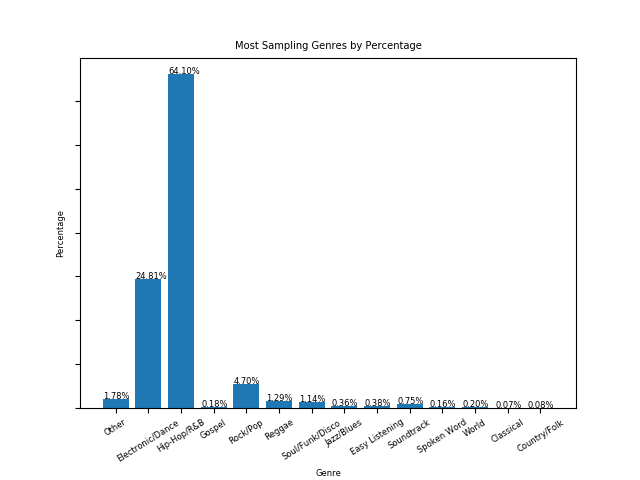
\includegraphics{topSamplingGenresPercent}
\caption{Most Sampling Genres Overall}
\label{fig:fig1}
% \label
\centering
\end{figure}
From Figure 1, Hip-Hop/R\&B artists make up 64.10\% of all artists that use samples in their music. The second highest sampling genre is Electronic/Dance with 24.81\% of all samples. Artists from these two genres alone make up 88.91\% of all music samplers throughout all musical history. In essence, Hip-Hop/R\&B is clearly the highest-volume music sampler in the music community compared to all other genres as originally claimed by the general public. 
\subsubsection{Did "Grand Upright Music Ltd. v. Warner Bros. Records Inc." slow the sampling trend?}
The landmark court case in 1991 placed the first set of federal sampling laws upon artists, theoretically dissuading future artists from utilizing sampling in their music as the process for receiving a clearance to use a sample is often not worth the time or within the budget of many artists.
\begin{figure}[H]
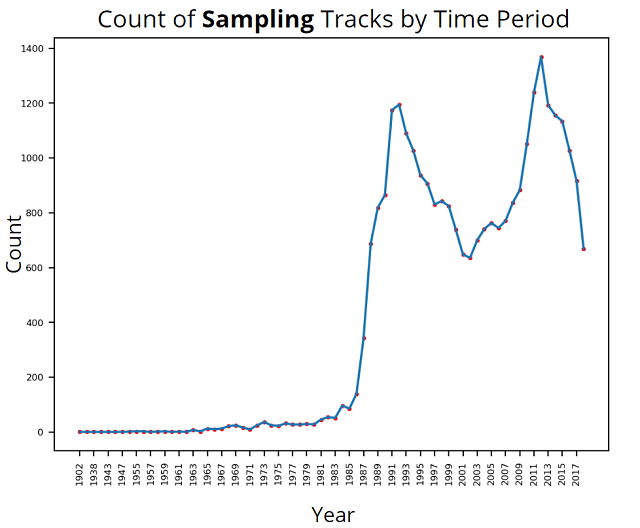
\includegraphics{TimePeriods/samplingTimePeriod}
\caption{Count of Sampling Tracks by Time Period}
\label{fig:fig2}
\centering
\end{figure}
As seen in Figure 2, sampling volume saw a huge downturn from having approximately 1200 songs (in the dataset) with samples in year 1991 to approximately 600 samples by 2001. Sampling volume clearly becomes wildly popular in the late 1980's before it abruptly drops around year 1991. This decrease in sampling volume occurs until 2001 when yearly sampling volume finally rises again until year 2011 when sampling volume equalizes the levels seen in 1991. 

There is a clear drop in sampling volume post-1991 that does not begin to recover for another decade around 2001 as indicated in Figure 2. While this is correlated with the year of the Grand Upright Music Ltd. v. Warner Bros. Records Inc. ruling, we cannot say that the downturn was a direct result of the ruling. However to answer the claim, we can say that the volume of sampling tracks post-1991 do correspond with a slowing in sampling usage in music overall.

As an aside, there is a large dip in sampling data post-2010. This can be attributed to the lack of sampling data from the 2010's in the WhoSampled database as mentioned in the Implementation.
\subsection{Most Influential Genres}
\begin{figure}[H]
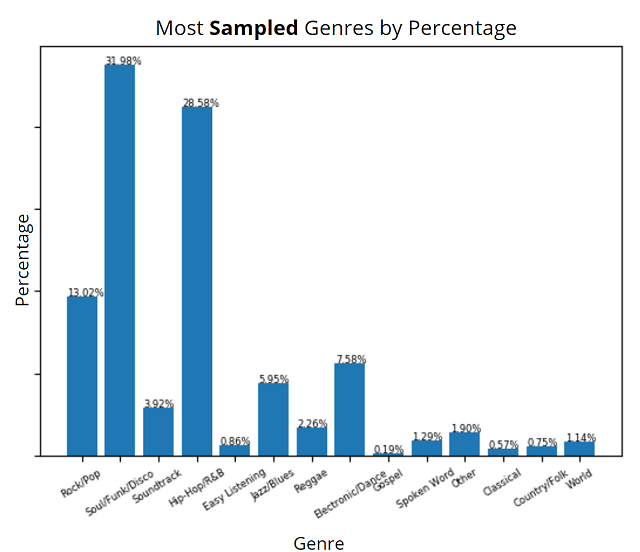
\includegraphics{topSampledGenresPercent}
\caption{Most Sampled Genres Overall}
\label{fig:fig3}
\centering
\end{figure}
Recall that greater influence is defined as being sampled by more artists. Analysis of influential genres entails considering the entire network and viewing the proportions of nodes with in-degrees greater than one followed by identifying these nodes by genre. The more nodes of a single genre that were sampled, the greater proportion of samples that came from that genre. In Figure 3, we see two genres that are deemed highly influential and are sampled above all other genres. Soul/Funk/Disco is the sampled genre of choice for 31.98\% of artists while Hip-Hop/R\&B is sampled 28.58\% of the time. It appears that Soul/Funk/Disco is slightly more influential as a genre than Hip-Hop/R\&B overall, but the two genres are clearly more influential than all other genres.
\begin{figure}[H]
\makebox[\textwidth]{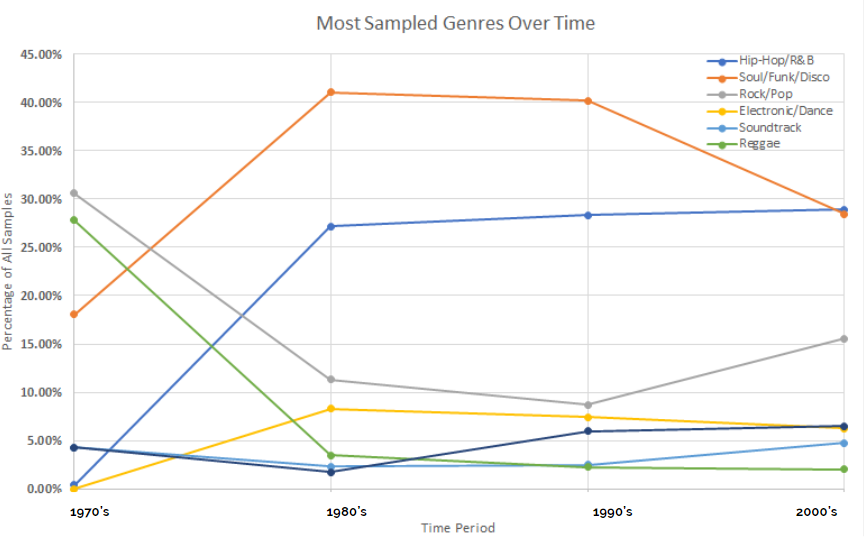
\includegraphics{./TimePeriods/mostSampledPlot}}
\caption{Most Sampled Genres Over Time}
\label{fig:fig4}
\centering
\end{figure}
From Figure 4, the early era of music sampling in the 1970's did not display a heavy influence by Soul/Funk/Disco or Hip-Hop/R\&B (which arguably was not invented at the time). Instead, Rock/Pop and Reggae were the genres of choice by samplers only to see a decline in every time period since the 1970's. From the 1980's onwards, Hip-Hop/R\&B and Soul/Funk/Disco established their strong influence. At its peak, Soul/Funk/Disco was sampled by over 40\% of all sampling artists in the 1980's before falling to under 30\% in the 2000's. Hip-Hop/R\&B's popularity as a sampled genre rose dramatically in the 1970's and has made steady, minor increases in sampled proportion since. By being sampled roughly 27\% of the time in the 1980's to 29\% of the time in the 2000's, it has stabilized while Soul/Funk/Disco's sampled proportion dropped. Hip-Hop/R\&B as of the 2000's has taken over as the most influential genre over Soul/Funk/Disco (by a very small margin). From this we can gather that the two aforementioned genres continue to be highly influential but Soul/Funk/Disco's influence may be lessening in the current and future time periods.
\subsection{Intra-genre and Inter-genre Sampling Strength}
Intra-genre sampling is a strong and insignificant factor when an artist decides to sample music. When viewing the entire dataset, 32.6\% of all samples by artists were found to be from other artists within their same genre. This is an insignificant proportion considering one might expect an artist to sample from all genres equally and uniformly. Clearly artists from a genre are inclined to sample from other artists in their genre as it may align more closely to the musical vision they are attempting to reach.
% This is where we perform the Chi Square confidence test and analyze the p-values between closely proportioned genres. The null hypothesis is that this distribution and the expected distribution (hip hop and soul are equally distributed) are the same.
\begin{figure}[H]
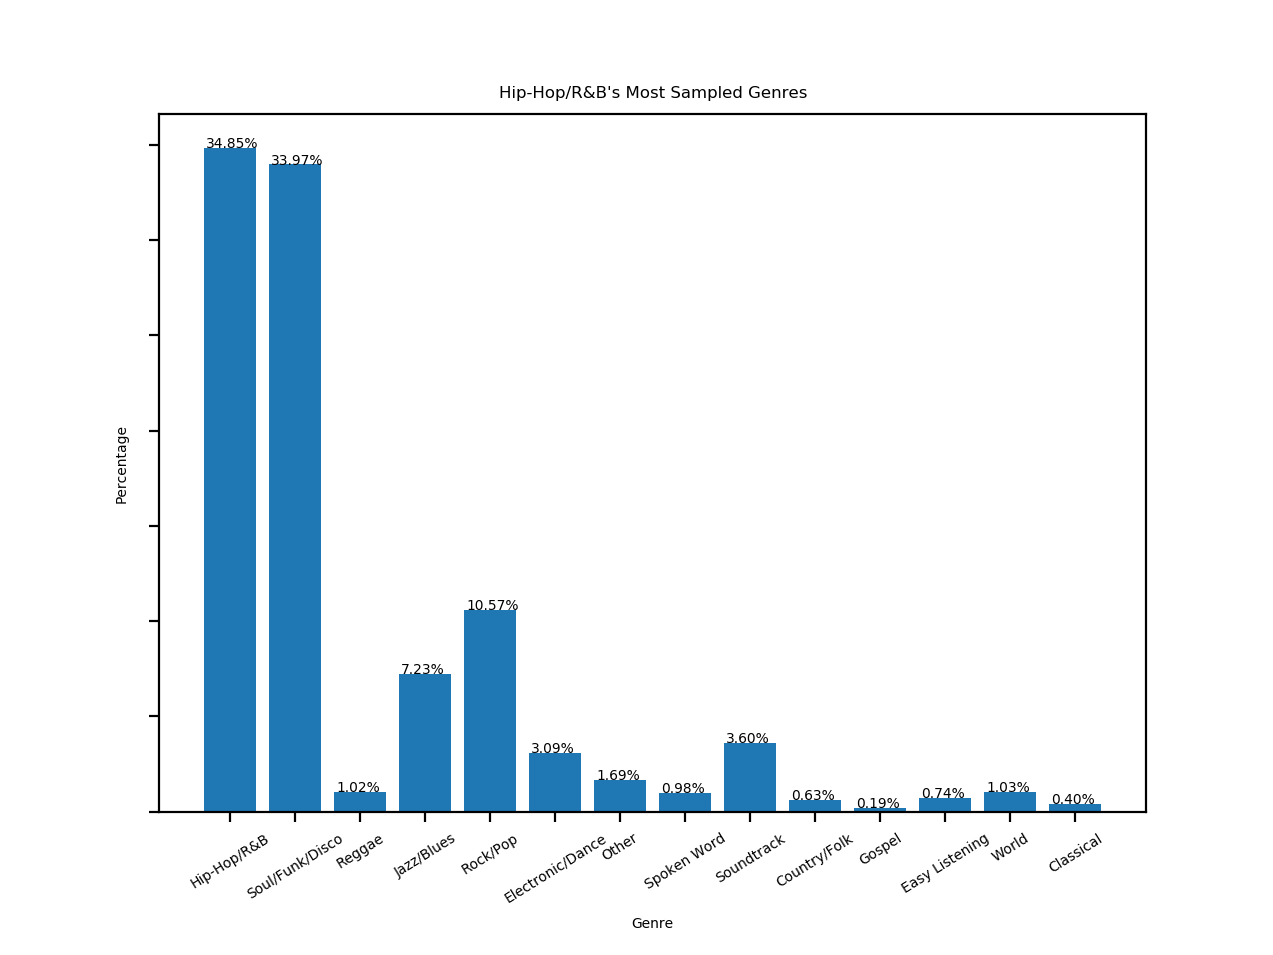
\includegraphics{./genreRatio/genreRatioHiphop}
\caption{Hip-Hop Sampling Proportions}
\label{fig:fig5}
\centering
\end{figure}
When viewing Figure 5's display of Hip-Hop Sampling Proportions, one can see that Hip-Hop/R\&B artists sample heavily from other artists in their genre as well as Soul/Funk/Disco artists. These two genres comprise over two-thirds of the genres sampled by Hip-Hop/R\&B artists. However, wouldn't one already expect this as Hip-Hop/R\&B and Soul/Funk/Disco are the two most influential genres in music as shown in the previous subsection?
\begin{figure}[H]
\makebox[\textwidth]{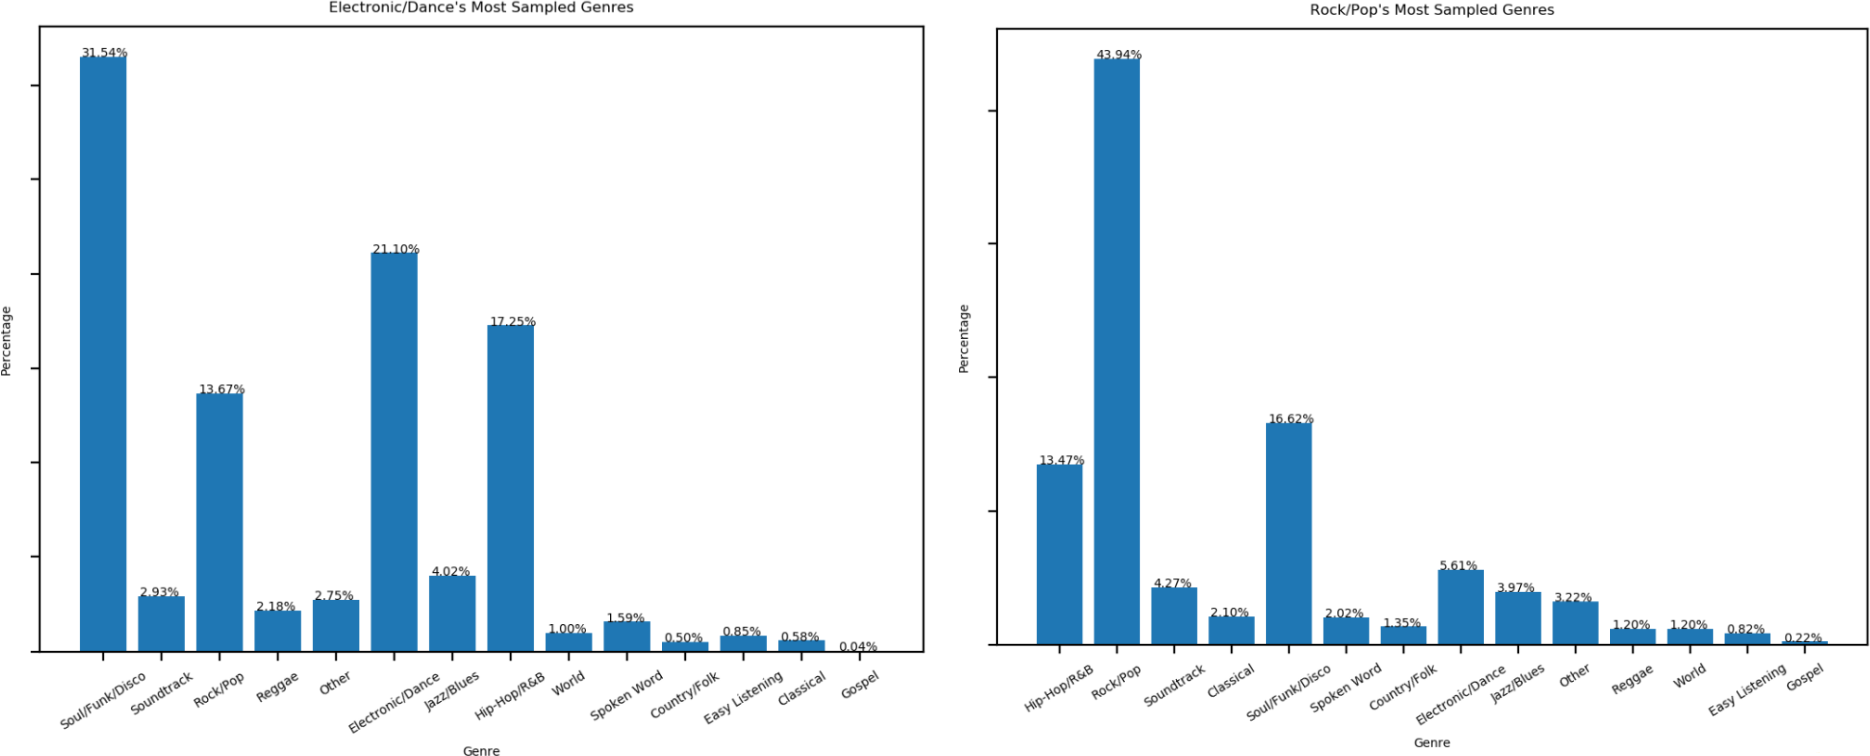
\includegraphics[scale=0.56]{./genreRatio/genreRatioElectronicRock}}
\centering
\caption{Electronic/Dance Sampling Proportions}\caption{Rock/Pop Sampling Proportions}
\label{fig:fig6}
\label{fig:fig7}
\end{figure}
Despite the strong genre influence of Hip-Hop/R\&B and Soul/Funk/Disco, we are able to observe the effects of artists to sample from within their genre in Figures 6 and 7. Electronic/Dance artists sample Soul/Funk/Disco the most (31.51\% of the time) and Hip-Hop/R\&B third-most (17.25\% of the time) but also sample their own genre second-most. We see this same effect as Rock/Pop artists sample other Rock/Pop artists the most (43.94\% of the time). This same pattern is observed in every other genre's intra-genre sampling proportions. Some genres display this effect more prominently than others.
\begin{figure}[H]
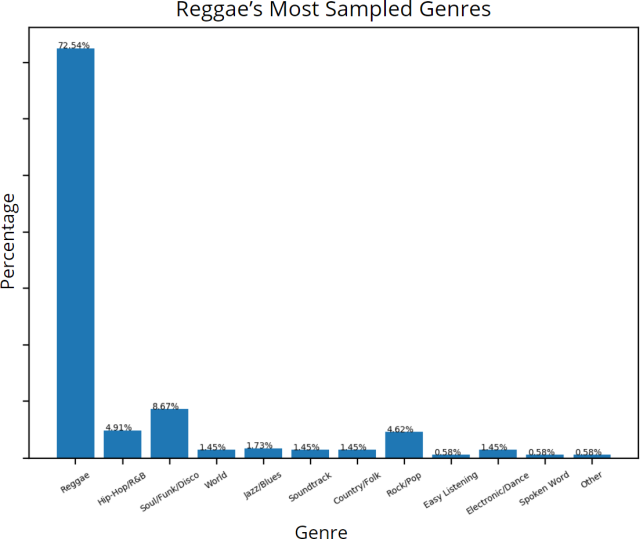
\includegraphics{./genreRatio/genreRatioReggae}
\caption{Reggae Sampling Proportions}
\label{fig:fig8}
\centering
\end{figure}
From Figure 8, 72.54\% of the samples found in Reggae are also by Reggae artists!
From these results it appears that it is quite common to observe artists sampling others in their genre despite the heavy influence of major sampled genres addressed in the previous subsection. 
\subsection{Patterns in Audio Element Sampling}
The inclusion of sampled audio elements allowed the attempt to derive patterns between genres, sampling time periods, and the specific types of audio elements chosen for samples. However, the reality of the dataset was a less-nuanced set of variables to describe audio elements than hoped.

If more than one audio element is sampled by a song, the audio element sampled is considered "Multiple Elements" rather than having the specific sampled audio elements listed. This leads to the inability to develop any noticeable strong correlations between combinations of audio elements that are sampled together by specific genres.
\begin{figure}[H]
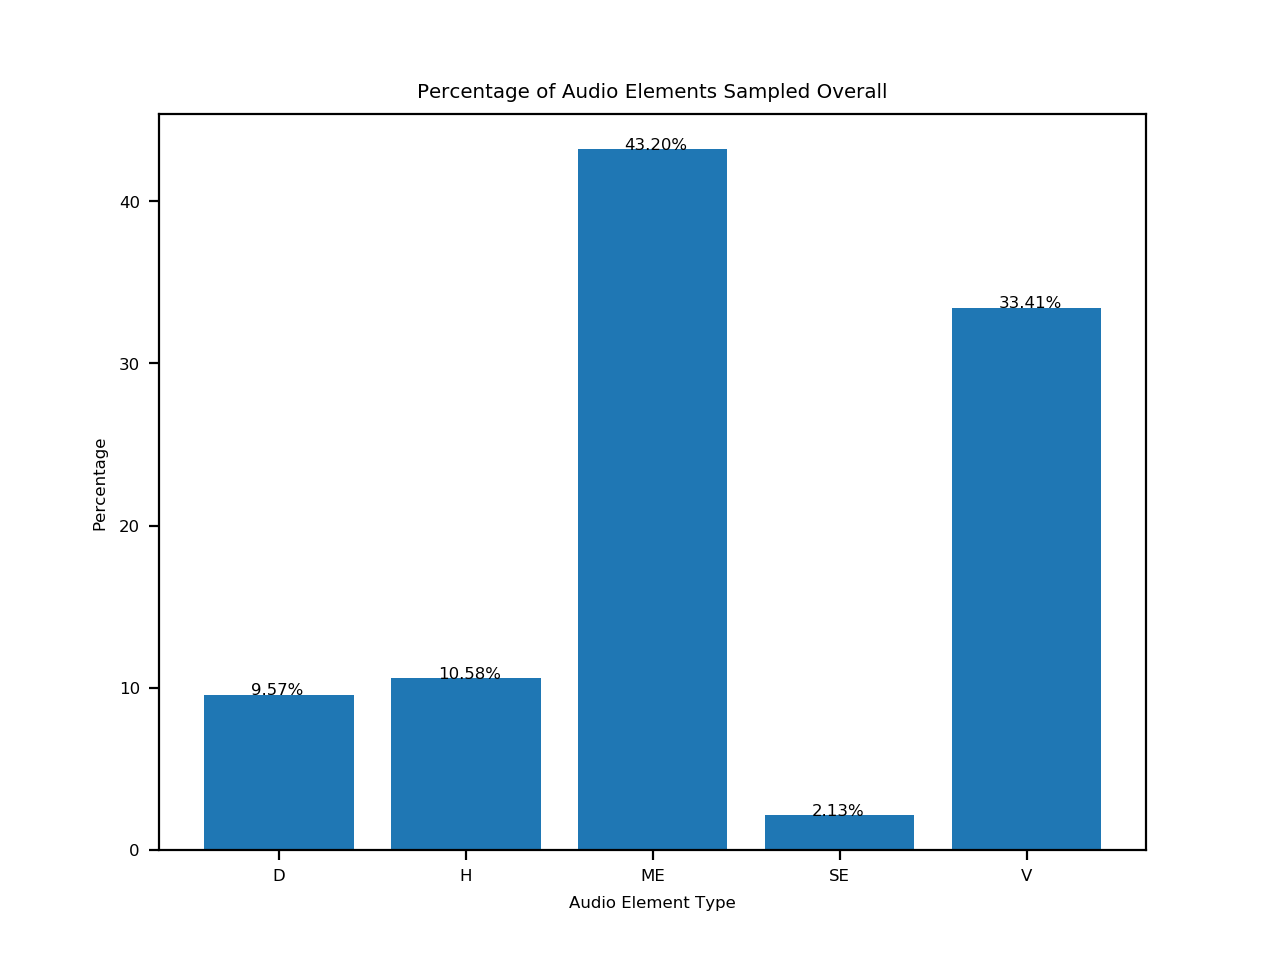
\includegraphics{audioElemSampledOverall}
\caption{Most Sampled Audio Elements Overall}
\label{fig:fig9}
\centering
\end{figure}
However, the analysis of audio elements did show that artists across all genres tend to have either Vocals alone or Multiple Elements sampled from their music. In Figure 9, 43.20\% of all audio elements sampled are Multiple Elements while 33.41\% are Vocals. 
\begin{figure}[H]
\makebox[\textwidth]{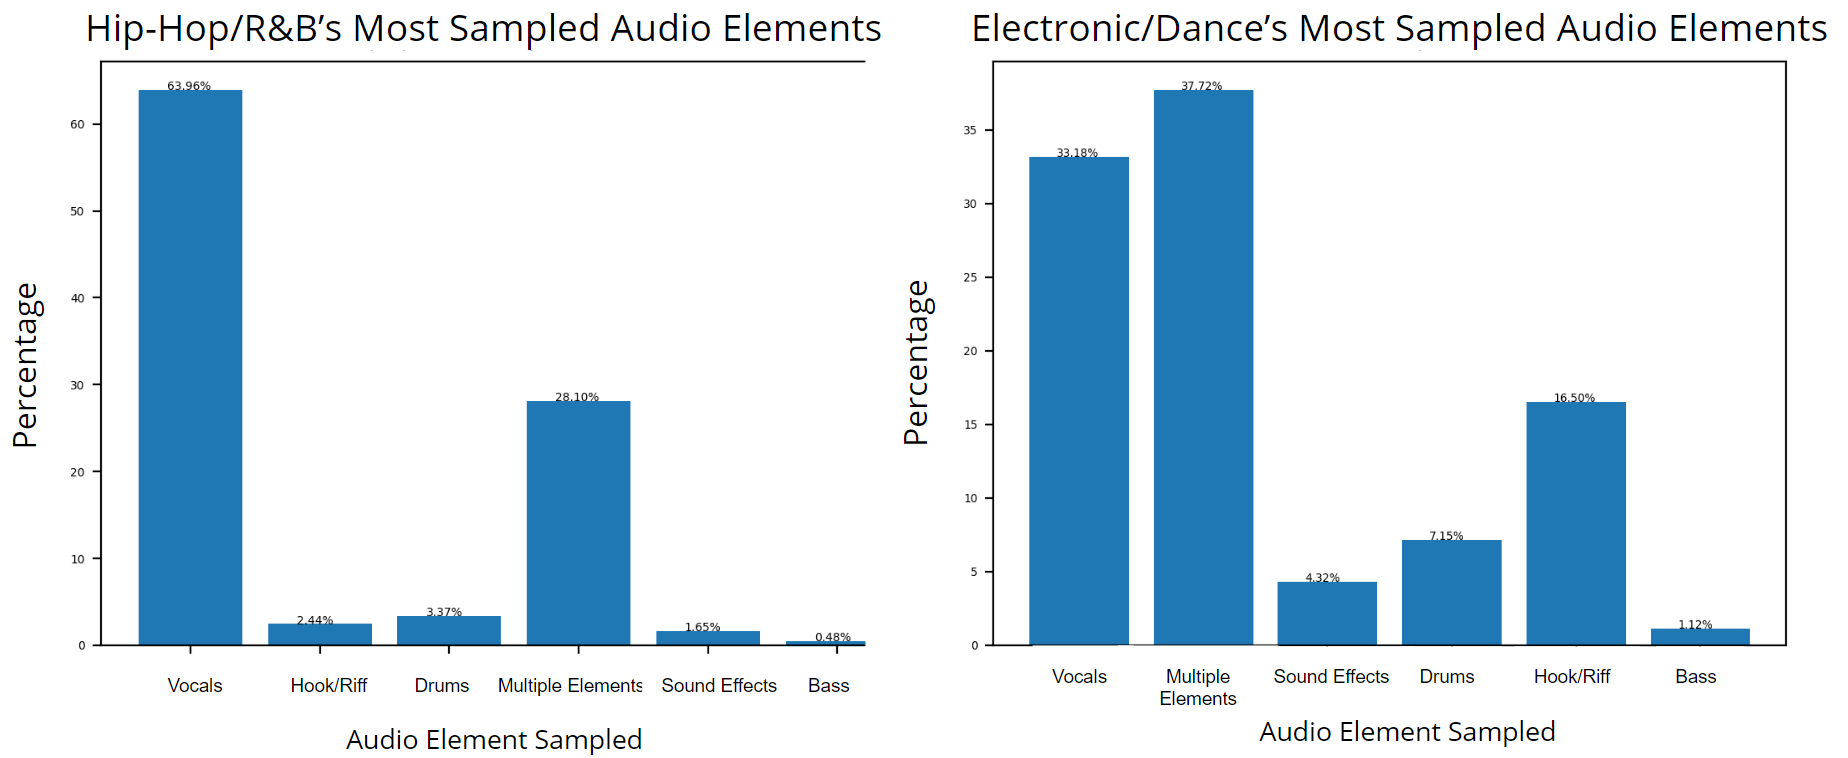
\includegraphics[scale=0.58]{./audioElemSampledBy/audioElemElectronicHip}}
\centering
\caption{Most Sampled Audio Elements by Hip-Hop/R\&B}\caption{Most Sampled Audio Elements by Electronic/Dance}
\label{fig:fig10}
\label{fig:fig11}
\end{figure}
Viewing the audio elements sampled by Hip-Hop/R\&B and Electronic/Dance (the top sampling genres), 46.13\% of audio elements that Hip-Hop/R\&B artists sample are Multiple Elements and 32.96\% are Vocals while 35.53\% of audio elements that Electronic/Dance artists sample are Multiple Elements and 35.30\% are Vocals. This follows the pattern in which Multiple Elements and Vocals are always the two most-sampled audio elements. This dominance of Multiple Elements and Vocals as sampled audio elements stands for every genre analyzed.

Though it is a weak result compared to what a more detailed dataset could have provided, the data appears to reflect a sampling pattern where artists across all genres either sample Multiple Elements of tracks or just Vocals.

Despite this failure to find a distinct audio element sampling pattern, it is clear that some artists have a specific element of their music sampled for distinct reasons. Take The Winstons and their widely sampled song "Amen Brother".
\begin{figure}[H]
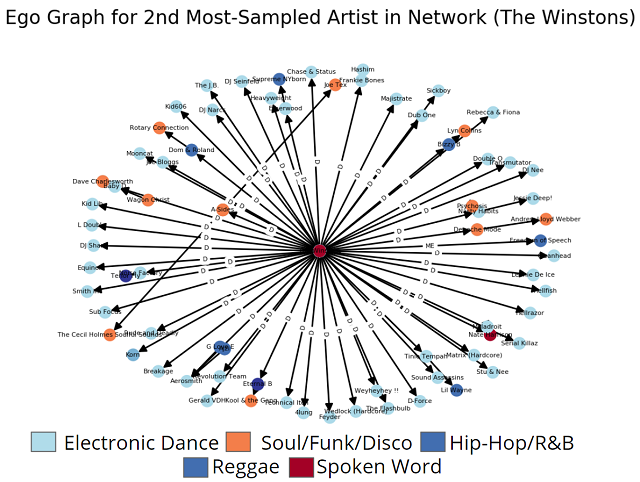
\includegraphics{./EgoGraphs/egoGraphMostSampled2TheWinstons}
\caption{The Winstons' Ego Graph}
\label{fig:fig12}
\centering
\end{figure}
As observed in the Ego Graph seen in Figure 12, nearly all existing samples of The Winstons are specifically Drum samples. Few other audio elements of their music is sampled. Despite this anomaly with The Winstons, general sampling patterns do not follow such a blatant sampling pattern and are much more varied as stated earlier.
\subsection{Most Influential Artists}
\begin{table}[H]
\resizebox{\textwidth}{!}{%
\begin{tabular}{|c|c|c|c|c|c|c|}
\hline
\textbf{Artist Rank} & \textbf{In-Degree Centrality} & \textbf{Betweenness Centrality} & \textbf{Closeness Centrality} & \textbf{Eigenvector Centrality} & \textbf{Katz Centrality} & \textbf{PageRank} \\ \hline
1. & James Brown (3.14E-2) & Public Enemy (4.48E-3) & James Brown (1.03E-1) & James Brown (0.53E-1) & James Brown (0.47E-1) & James Brown (1.74E-2) \\ \hline
2. & The Winstons (1.62E-2) & Beastie Boys (4.35E-3) & Lyn Collins (0.85E-1) & LL Cool J (0.23E-1) & Public Enemy (0.18E-1) & Lyn Collins (0.74E-2) \\ \hline
3. & Public Enemy (1.41E-2) & LL Cool J (4.15E-3) & The J.B.'s (0.78E-1) & Run-DMC (0.22E-1) & Lyn Collins (0.17E-1) & Afrika Bambaataa (0.51E-2) \\ \hline
4. & Lyn Collins (1.21E-2) & De La Soul (3.83E-3) & Fred Wesley (0.77E-1) & Lyn Collins (0.19E-1) & Run-DMC (0.16E-1) & Public Enemy (0.47E-2) \\ \hline
5. & Beside (1.07E-2) & Jay-Z (3.49E-3) & Beside (0.67E-1) & Public Enemy (0.18E-1) & LL Cool J (0.14E-1) & The Winstons (0.47E-2) \\ \hline
\end{tabular}%
}
\caption{Top Artist Centralities (All Time Periods)}
\label{table:table1}
\end{table}
Over all time periods, it is important to note the strong presence of James Brown in every centrality measure except for betweenness centrality. Recall that betweenness centrality only refers to the ability of an artist to "bridge" communities due to the samples they use in their music or the music that samples them. Therefore an artist like Public Enemy that is sampled by a diverse set of artists from different genres and sample others in high volumes would display a high betweenness centrality.

Aside from James Brown's missing presence in Betweenness Centrality, he is ranked in the number one position in every other centrality ranking indicating his great influence in  each of the ways centrality can be measured. 

Also note that nearly every artist displayed in the table is a Soul/Funk/Disco or Hip-Hop/R\&B artist, further confirming that the these are the two most influential genres in music.
\begin{table}[H]
\resizebox{\textwidth}{!}{%
\begin{tabular}{|c|c|c|c|c|c|c|}
\hline
\textbf{Artist Rank} & \textbf{In-Degree Centrality} & \textbf{Betweenness Centrality} & \textbf{Closeness Centrality} & \textbf{Eigenvector Centrality} & \textbf{Katz Centrality} & \textbf{PageRank} \\ \hline
1. & James Brown (8.73E-2) & Public Enemy (5.15E-4) & James Brown (1.22E-1) & James Brown (4.49E-1) & James Brown (3.88E-1) & James Brown (5.49E-2) \\ \hline
2. & Beside (3.77E-2) & Kurtis Blow (3.05E-4) & The J.B.'s (8.43E-2) & John Davis and the Monster Orchestra (3.39E-1) & Beside (1.56E-1) & Fred Wesley (1.69E-2) \\ \hline
3. & Run-DMC (2.40E-2) & Beastie Boys (3.05E-4) & Fred Wesley (8.31E-2) & Kurtis Blow (3.99E-1) & Run-DMC (1.27E-1) & The J.B.'s (1.67E-2) \\ \hline
4. & Public Enemy (2.23E-2) & Run-DMC (2.74E-4) & Beside (5.98E-2) & Run-DMC (3.99E-1) & Kurtis Blow (1.06E-1) & Afrika Bambaataa (1.60E-2) \\ \hline
5. & Kurtis Blow (1.60E-2) & James Brown (2.53E-4) & Afrika Bambaataa (5.23E-2) & The J.B.'s (2.23E-1) & Public Enemy (1.04E-1) & Beside (1.40E-2) \\ \hline
\end{tabular}%
}
\caption{Top Artist Centralities (1980's)}
\label{table:table2}
\end{table}
\begin{table}[H]
\resizebox{\textwidth}{!}{%
\begin{tabular}{|c|c|c|c|c|c|c|}
\hline
\textbf{Artist Rank} & \textbf{In-Degree Centrality} & \textbf{Betweenness Centrality} & \textbf{Closeness Centrality} & \textbf{Eigenvector Centrality} & \textbf{Katz Centrality} & \textbf{PageRank} \\ \hline
1. & James Brown (5.39E-2) & Public Enemy (7.25E-3) & James Brown (1.04E-1) & James Brown (5.42E-1) & James Brown (4.26E-1) & James Brown (2.51E-2) \\ \hline
2. & Public Enemy (2.27E-2) & Masta Ace Incorporated (4.76E-3) & Lyn Collins (8.68E-2) & Lyn Collins (2.69E-1) & Public Enemy (1.76E-1) & Lyn Collins (1.21E-2) \\ \hline
3. & The Winstons (1.95E-2) & LL Cool J (3.65E-3) & Fred Wesley (7.93E-2) & Fred Wesley (2.22E-1) & Lyn Collins (1.63E-1) & Fred Wesley (8.86E-3) \\ \hline
4. & Lyn Collins (1.57E-2) & Beastie Boys (3.58E-3) & Melvin Bliss (6.13E-2) & Parliament (1.99E-1) & N.W.A. (1.32E-1) & Public Enemy (7.86E-3) \\ \hline
5. & Run-DMC (1.40E-2) & De La Soul (3.46E-3) & Parliament (6.01E-2) & LL Cool J (1.98E-1) & Run-DMC (1.28E-1) & The Winstons (6.69E-3) \\ \hline
\end{tabular}%
}
\caption{Top Artist Centralities (1990's)}
\label{table:table3}
\end{table}
\begin{table}[H]
\resizebox{\textwidth}{!}{%
\begin{tabular}{|c|c|c|c|c|c|c|}
\hline
\textbf{Artist Rank} & \textbf{In-Degree Centrality} & \textbf{Betweenness Centrality} & \textbf{Closeness Centrality} & \textbf{Eigenvector Centrality} & \textbf{Katz Centrality} & \textbf{PageRank} \\ \hline
1. & James Brown (9.95E-3) & Jay-Z (4.42E-4) & The Notorious B.I.G.(2.74E-2) & The Notorious B.I.G. (3.48E-1) & The Notorious B.I.G. (1.04E-1) & Run-DMC (6.56E-3) \\ \hline
2. & The Winstons (9.82E-3) & Public Enemy (3.81E-4) & James Brown (2.59E-2) & Public Enemy (3.28E-1) & James Brown (9.90E-2) & Public Enemy (3.68E-3)\\ \hline
3. & The Notorious B.I.G. (8.20E-3) & Kanye West (3.61E-4) & Public Enemy (2.52E-2) & EPMD (2.64E-1) & Public Enemy (8.79E-2) & The Notorious B.I.G. (3.64E-3) \\ \hline
4. & Beside (8.20E-3) & 50 Cent (3.20E-4) & Beside (2.44E-2) & Run-DMC (2.49E-1) & Beside (8.36E-2) & James Brown (3.52E-3)\\ \hline
5. & Public Enemy (6.86E-3) & Nas (3.07E-4) & Run-DMC (2.37E-2) & James Brown (2249E-1) & The Winstons (8.16E-2) & Beside (3.51E-3) \\ \hline
\end{tabular}%
}
\caption{Top Artist Centralities (2000's)}
\label{table:table4}
\end{table}
Note that 19 of the 20 artists in the betweenness centrality ranking tables are Hip-Hop/R\&B artists except for James Brown, a Soul/Funk/Disco artist. This reflects the earlier statement that states Hip-Hop/R\&B artists in general are sampled by a diverse set of artists from different genres and sample in higher volumes leading to a higher betweenness centrality.

Also notice that James Brown's domination of the centrality rankings in each time period weakens in the 2000's (seen in Table 4) as he is relegated to positions below rank 1. Though he still appears in the top 5 of every centrality measure (besides betweenness centrality), it appears that his influence lessens in the modern sampling environment. The music sampling community in the 2000's appears to be centralized greatly around more Hip-Hop/R\&B artists such as The Notorious B.I.G. But, this should come as no surprise as one can observe Figure 4 which depicts the weakening hold of Soul/Funk/Disco samples in the 2000's as it is replaced by Hip-Hop/R\&B.

Despite this lowered ranking for James Brown in the 2000's, his appearance in nearly every top 5 temporal centrality ranking over the time periods indicates his strong influence. The only other artists that appear in each of these time periods as well as the overall centrality ranking are Public Enemy and Run-DMC. This indicates that these artists have strong sampling influence over many time periods and continue to be sampled as music sampling practices may change.
\subsection{Average Clustering Coefficients}
Over all time periods, the average clustering coefficient for the entire graph appears to be extremely small indicating that groups of samplers tend to be small and are rarely tight-knit about an artist or set of artists. Of course with a large number of nodes, one might expect the average clustering coefficient to be quite low.
\begin{table}[H]
\centering
\begin{tabular}{|c|c|}
\hline
\textbf{Time Period} & \textbf{Average Clustering Coefficient} \\ \hline
Overall & 0.003854434 \\ \hline
1980's & 0.004470729 \\ \hline
1990's & 0.003857424 \\ \hline
2000's & 0.001085667 \\ \hline
\end{tabular}
\caption{Average Local Clustering Coefficients Over Time}
\label{table:table5}
\end{table}
Reffering to Table 5, the change in the clustering coefficient appears to decrease from the 1980's to the 2000's but the absolute change in the clustering coefficient is small for the overall musical sampling community. The low clustering coefficient overall demonstrates the tendency for artists to not cluster together with all other artists in the network. Because of the nature of sampling data and the wide variety of artists a single artist could possibly sample from, a low average clustering coefficient is not unexpected. However, the trend of a lowering average clustering coefficient over time means artists tend to form fewer tightly knit groups that sample primarily from each other, possibly indicating artists sampling from unique artists that are not widely sampled by others.
\subsection{Louvain Communities}
\begin{table}[H]
\resizebox{\textwidth}{!}{%
\begin{tabular}{|c|c|c|c|c|c}
\cline{1-5}
\textbf{n'th Largest Louvain Community} & \multicolumn{4}{c|}{\textbf{Genre (\% in n'th Largest Community)}} &  \\ \cline{1-5}
\textbf{} & {\ul Hip-Hop/R\&B} & {\ul Electronic/Dance} & {\ul Rock/Pop} & {\ul Soul/Funk/Disco} &  \\ \cline{1-5}
1. & 55.56\% & 14.23\% & 10.35\% & 7.46\% &  \\ \cline{1-5}
2. & 59.68\% & 20.45\% & 5.56\% & 7.44\% &  \\ \cline{1-5}
3. & 56.84\% & 19.04\% & 6.64\% & 8.11\% &  \\ \cline{1-5}
4. & 55.57\% & 14.06\% & 7.29\% & 9.42\% &  \\ \cline{1-5}
5. & 12.20\% & 60.59\% & 8.71\% & 2.41\% &  \\ \cline{1-5}
\end{tabular}%
}
\caption{Top Genre Makeup in n'th Largest Louvain Communities}
\label{table:table6}
\end{table}
The proportional makeup of each of the largest Louvain communities came to an unsurprising conclusion given our observations with intra-genre sampling: Each of the partitioned communities were dominated by a single genre. For four of the five largest Louvain communities, Hip-Hop/R\&B was the genre making up the majority of the community as observed in Table 6. Electronic/Dance came 2nd to Hip-Hop/R\&B in each of these 4 communities and was the most prevalent genre in the 5th largest Louvain community.

This single-genre dominance is the result of a genre that has a high sampling volume in its music. Based on our results from investigating intra-genre sampling, this same genre with high sampling volume frequently samples from artists within its own genre which leads to an insular Louvain community.
\begin{figure}[H]
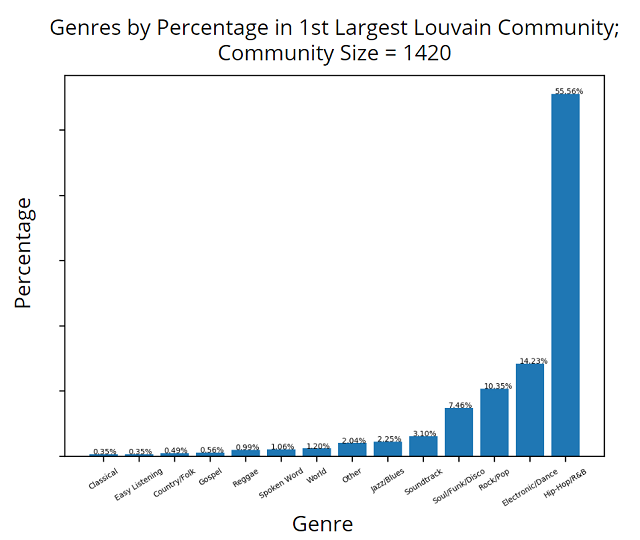
\includegraphics{LouvainCommunities/louvain1st}
\caption{Genre Makeup of Largest Louvain Community}
\label{fig:fig13}
\centering
\end{figure}
As shown in Figure 13, 55.56\% of artists in the largest Louvain Community are Hip-Hop/R\&B artists, indicating a high level of intra-level sampling and an insular sampling pattern. The most prevalent genres in this community are a combination of the top sampling genres and the most sampled genres over all time periods. Genres that are found most often in the Louvain communities are those that have a greater presence in the sampling community either by being sampled by many artists or by sampling many artists themselves.
\section{Conclusion and Future Work}
\subsection{Conclusion}
Through network analysis of the sampling network, we first verified the historical musical sampling claims perpetuated in modern media and found them to be quantitatively verified. Hip-Hop/R\&B does sample music dramatically more often than other genres with Electronic/Dance following it. Though we couldn't form a causative relationship between the sampling laws that arose from "Grand Upright Music Ltd. v. Warner Bros. Records Inc." and the decrease in sampling volume in 1991, there was a noticeable correlation in the period after 1991 with a decreased sampling volume.

We then analyzed the dataset for the most influential genres which are the genres sampled the most often by artists. Soul/Funk/Disco was the most influential genre overall but Hip-Hop/R\&B has recently challenged this. After performing a temporal analysis, it appears that Hip-Hop/R\&B has consistently been sampled by artists 25-30\% of the time while Soul/Funk/Disco has seen a decrease in the proportion of sampled genres since the 1980's.

Intra-genre influences were found to be strong and artists noticeably sampled from other artists within their genre just as much as they sampled from the most influential genres (if not more). Some genres displayed higher proportions of intra-genre sampling but the greatest takeaway was that all genres do show a strong tendency to sample from within their genre.

James Brown was and continues to be one of the most influential artists throughout all eras of music as indicated by numerous types of centrality measurements. He is without a doubt the most influential artist but other artists such as Public Enemy and Run-DMC also display just as strong of influence overall and throughout all time periods of music. Centrality measurements also reinforced the strength of Hip-Hop/R\&B and Soul/Funk/Disco as the most influential genres in music sampling.

The average clustering coefficient of the entire network was found to be very low throughout all time periods as expected due to the nature of music sampling. After all, an artist is unlikely to sample from many pieces of the music in the 30,000 point dataset. However, a decrease in the average clustering coefficient over time periods since the 1980's may indicate fewer tightly knit groups of artists that sample primarily from each other.

Louvain communities also helped reinforce the notion of strong intra-genre sampling and the dominance of Hip-Hop/R\&B and Electronic/Dance as the highest volume samplers across all genres of music. By being highly sampling genres found in these communities, their majority proportion in each of the largest Louvain communities occurred as a result of strong intra-genre sampling. The more Hip-Hop/R\&B or Electronic/Dance samplers are in a community, the more they sample from their own genre resulting in a compounding effect.

The greatest limitation in the analysis of the sampling network was the lack of granularity in the Audio Element property of the WhoSampled dataset. Due to the labelling scheme in which the sampling of multiple audio elements leads to a sample being categorized as "Multiple Elements" rather than listing each of the audio elements, we were unable to notice any patterns that arose from certain genres or time periods. The only conclusion that could be drawn was that artists tend to sample Vocals if they do not sample Multiple Elements.

Another limitation stemming from the dataset was the lack of sampling data for music released in the 2010's. Much of the sample data in the dataset was concentrated in the 1980's-2000's. Though these eras are indicative of the peak in sampling popularity as a musical device, it is unclear if the data for the most recent decade is lacking due to lack of valid data or actual lack of sampling in the music community. As a result, we did not perform temporal analysis on this time period. Future research could be performed at a later date to observe if the data for this time period is entered into WhoSampled.
\subsection{Future Work}
Future studies of musical sampling influence networks can look towards the patterns established by this paper to create an application capable of making predictions about the types of samples likely to be found in a song containing the specific defining characteristics we researched in this project. This predictive analysis could potentially aid developers such as WhoSampled with their music sampling identification software by acting as a false positive check.

From a legal perspective, the sampling patterns that establish the potential for a predictive algorithm could be used for ground truth facts during legal proceedings of musical sampling lawsuits. There are often initial arguments from parties debating whether a song was actually sampled by another song and a predictive algorithm could help determine the likelihood this is true based on an artist's past behaviors within the current musical community's trends.

Legal and historical scholars could also perform a deeper analysis of the dip in sampling volume post-1991 that is correlated with the Grand Upright Music v. Warner Bros. Records copyright case that famously ruled the specifics behind what constitutes a legal sample.
\section{Acknowledgments}
I would like to thank Professor Andrea LaPaugh for organizing the Network Analysis Independent Work seminar and advising this project. I would also like to thank Bobray J. Bordelon and Darwin F. Scott of the Princeton University Library for enabling access to the WhoSampled Academic Pro dataset.
\nocite{*}
\bstctlcite{bstctl:etal, bstctl:nodash, bstctl:simpurl}
\bibliographystyle{IEEEtranS}
\bibliography{references}

\end{document}